\documentclass[10pt, letterpaper]{report}
% !TeX program = xelatex
%==================PREAMBOLO=======================%
\usepackage[utf8]{inputenc}
\usepackage{psvectorian}
\usepackage{pgfplots}
\usepackage[Rejne]{fncychap}
\usepackage[export]{adjustbox}
\usepackage[T1]{fontenc}
\usepackage{lmodern}
\usepackage{blindtext}
\usepackage{pdfpages}
\usepackage[shortlabels]{enumitem}
\usepackage{moresize}
\usepackage{graphicx} % Required for inserting images
\usepackage{hyperref}
\usepackage{listings}
\usepackage[table,xcdraw]{xcolor}
\usepackage{amssymb}
\usepackage{amsmath}
\usepackage[english]{babel}
\usepackage{nicefrac, xfrac}
\usepackage{tikz}
\usepackage{tikz-3dplot}
\usepackage{tikz-cd}
\usepackage{mathrsfs} 
\usepackage{titletoc}
\usepackage{fancyhdr}
\usepackage{psvectorian,lipsum}
\usepackage{fourier-orns}
\usepackage{lipsum}
\usepackage{wrapfig}
\usepackage{multicol}
\usepackage[paper=a4paper,left=25mm,right=25mm,bottom=25mm,top=25mm]{geometry}
\definecolor{light-gray}{gray}{0.95}
\definecolor{cop}{HTML}{f7ecd7}
\definecolor{copAut}{HTML}{ababab}
\definecolor{copAut2}{HTML}{c3c3e6}
\definecolor{purcop}{HTML}{d0d3db}
\definecolor{sapienza}{HTML}{660f1d}
\definecolor{lightSapienza}{HTML}{e3d3d5}
\definecolor{darkgreen}{HTML}{008000}
\definecolor{cartaRiciclata}{HTML}{fcfcf7}
\newcommand{\redText}[1]{\color{red}#1\color{black}}
\newcommand{\code}[1]{\colorbox{light-gray}{\texttt{#1}}}
\newcommand{\codee}[1]{\colorbox{white}{\texttt{#1}}}
\newcommand{\K}{{\mathbb K}}
\newcommand{\notimplies}{%
  \mathrel{{\ooalign{\hidewidth$\not\phantom{=}$\hidewidth\cr$\implies$}}}}
\newcommand{\flowerLine}{ \begin{center}\decofourleft\hphantom{ }\decoone\hphantom{ }\decofourright\hphantom{}\hphantom{aa}
\decofourleft\hphantom{ }\decoone\hphantom{ }\decofourright\hphantom{}\hphantom{aa}
\decofourleft\hphantom{ }\decoone\hphantom{ }\decofourright\hphantom{}\hphantom{aa}
\decofourleft\hphantom{ }\decoone\hphantom{ }\decofourright\hphantom{}\hphantom{aa} 
\decofourleft\hphantom{ }\decoone\hphantom{ }\decofourright\hphantom{}\hphantom{aa}
\decofourleft\hphantom{ }\decoone\hphantom{ }\decofourright\hphantom{}\hphantom{aa}
\decofourleft\hphantom{ }\decoone\hphantom{ }\decofourright\hphantom{}\hphantom{aa}
\decofourleft\hphantom{ }\decoone\hphantom{ }\decofourright\hphantom{}\hphantom{aa}
\decofourleft\hphantom{ }\decoone\hphantom{ }\decofourright\hphantom{}\hphantom{aa}
\end{center}}
\definecolor{g}{RGB}{60, 50, 50}
\newcommand{\textg}[1]{\color{g}{\textbf{#1}}\color{black}}
\newcommand{\teo}[1]{{\large\color{sapienza}\textbf{Teorema #1 :\hphantom{a}}}}
\newcommand{\defi}[1]{{\large\color{sapienza}\textbf{Definizione #1 :\hphantom{a}}}}
\newcommand{\claim}[1]{{\color{sapienza}\textbf{Claim #1 :\hphantom{a}}}}
\newcommand{\lemma}[1]{{\color{sapienza}\textbf{Lemma #1 :\hphantom{a}}}}
\newcommand{\dimo}[1]{{\color{sapienza}\textbf{Dimostrazione #1 :\hphantom{a}}}}
\newcommand{\prop}[1]{{\color{sapienza}\textbf{Proposizione #1 :\hphantom{a}}}}
\newcommand\greybox[1]{%
  \vskip\baselineskip%
  \par\noindent\colorbox{light-gray}{%
    \begin{minipage}{\textwidth}#1\end{minipage}%
  }%
  \vskip\baselineskip%
}
\newcommand\sapbox[1]{%
  \vskip\baselineskip%
  \par\noindent\colorbox{lightSapienza}{%
    \begin{minipage}{\textwidth}#1\end{minipage}%
  }%
  \vskip\baselineskip%
}
\newcommand{\ridFunc}{{f:\Sigma^*\rightarrow \Sigma^*}}
\newcommand{\rid}{{\le_m^P}}
\newcommand{\Z}{{\mathbb Z}}
\newcommand{\blank}{{\sqcup}}
\newcommand{\Prob}{{\mathbb P}}
\newcommand{\R}{{\mathbb R}}
\newcommand{\VA}{{\mathbb E}}
\newcommand{\N}{{\mathbb N}}
\newcommand{\quat}{{\mathbb H}}
\newcommand{\C}{{\mathbb C}}
\newcommand{\Sn}{{\mathcal S_n}}
\newcommand{\An}{{\mathcal A_n}}
\newcommand{\E}{{\mathcal E}}
\newcommand{\B}{{\mathcal B}}
\newcommand{\mcm}{{\text{mcm}}}
\newcommand{\rg}{{\text{rg}}}
\newcommand{\ve}{{\bar v}}
\newcommand{\spaz}{{\text{\hphantom{aa}}}}
\newcommand{\MCD}{{\text{MCD}}}
\newcommand{\tc}{{\text{ tale che }}}
\newcommand{\supp}{{\text{Supp}}}
\newcommand{\acc}{\\\hphantom{}\\}
\newcommand{\esempio}[1]{{\acc\large\color{sapienza}\textbf{Esempio #1 \hphantom{a}}\acc}}
\newcommand{\bra}[1]{\langle #1 \rangle}
\newcommand{\aut}{{\text{Aut}}}
\newcommand{\Span}{{\text{Span}}}
\newcommand{\End}{{\text{End}}}
\newcommand{\cen}{{\text{Centro}}}
\newcommand{\norm}{{\unlhd}}
\newcommand{\ciclS}{{\left \langle }}
\newcommand{\ciclE}{{\right \rangle }}
\newcommand{\boxedMath}[1]{\begin{tabular}{|c|}\hline \texttt{#1} \\ \hline\end{tabular} :} 
\newcommand{\shell}[1]{\colorbox{black}{\textcolor{white}{\texttt{#1}}}}
\newcommand{\eqImportante}[1]{\begin{center}\huge\lefthand\hphantom{a}
    \normalsize\texttt{#1}
    \hphantom{aaa}\huge\righthand\end{center}}

\fancyhf{}
\pagestyle{fancy}
\usepackage{pgf-pie}  
\usetikzlibrary{positioning}

\renewcommand{\headrule}{%
\vspace{-8pt}\hrulefill
\raisebox{-2.1pt}{\quad\decothreeleft\decotwo\decothreeright\quad}\hrulefill}

%sta roba serve per il codice C
\definecolor{mGreen}{rgb}{0,0.6,0}
\definecolor{mGray}{rgb}{0.5,0.5,0.5}
\definecolor{mPurple}{rgb}{0.58,0,0.82}
\definecolor{backgroundColour}{rgb}{0.95,0.95,0.92}

\lstdefinestyle{CStyle}{
    backgroundcolor=\color{backgroundColour},   
    commentstyle=\color{mGreen},
    keywordstyle=\color{magenta},
    numberstyle=\tiny\color{mGray},
    stringstyle=\color{mPurple},
    basicstyle=\footnotesize,
    breakatwhitespace=false,         
    breaklines=true,                 
    captionpos=b,                    
    keepspaces=true,                 
    numbers=left,                    
    numbersep=5pt,                  
    showspaces=false,                
    showstringspaces=false,
    showtabs=false,                  
    tabsize=2,
    language=C
}
\lstdefinestyle{CppStyle}{
    backgroundcolor=\color{backgroundColour},   
    commentstyle=\color{mGreen}\ttfamily,
    morecomment=[l][\color{magenta}]{\#}
    keywordstyle=\color{blue}\ttfamily,
    numberstyle=\tiny\color{mGray},
    stringstyle=\color{red}\ttfamily,
    basicstyle=\ttfamily,
    breakatwhitespace=false,         
    breaklines=true,                 
    captionpos=b,                    
    keepspaces=true,                 
    numbers=left,                    
    numbersep=5pt,                  
    showspaces=false,                
    showstringspaces=false,
    showtabs=false,                  
    tabsize=2,
    language=C
}
\lstset{language=C++,
                basicstyle=\ttfamily,
                keywordstyle=\color{blue}\ttfamily,
                stringstyle=\color{red}\ttfamily,
                commentstyle=\color{green}\ttfamily,
                morecomment=[l][\color{magenta}]{\#}
}
%fine roba che serve per il codice C
\usepackage{minted}
\usepackage{algorithm}
\usepackage{algpseudocode}
\newcommand{\titolo}{Artificial intelligence }

 %TOGLI COMMENTO SE USI XELATEX
%\usepackage{fontspec}
\title{\titolo} %========TITOLO========%
\author{Marco Casu}
\date{\vspace{-5ex}}
\begin{document}

%==================COPERTINA=======================%
\begin{titlepage}
    
\begin{center}
    %TOGLI COMMENTO SE USI XELATEX
   %\setmainfont{Palace Script MT}
   \HUGE Marco Casu\acc
\end{center}
\thispagestyle{empty}
\begin{figure}[h]
    \centering{
        %l'immagine deve avere una risoluzione 2048x2048
        
\includegraphics[width=1\textwidth ]{images/Copertina.png}
    }
\end{figure}
\vfill 
\centering 
\includegraphics[width=0.4\textwidth ]{../../preamble/Stemma_sapienza.png} \acc
\centering \Large \color{sapienza}Faculty of Information Engineering, Computer Science and Statistics\\
Department of Computer, Control and Management Engineering\\
Master's degree in Artificial Intelligence and Robotics
\end{titlepage}

%===================FINE COPERTINA======================%
\newpage
%\pagecolor{cartaRiciclata}%\setmainfont{Algerian}
\Large
This document summarizes and presents the topics for the \titolo course for the Master's degree in Artificial Intelligence and Robotics at Sapienza University of Rome. The document is free for any use. If the reader notices any typos, they are kindly requested to report them to the author.
\vfill
\begin{figure}[h!]
    \raggedright
    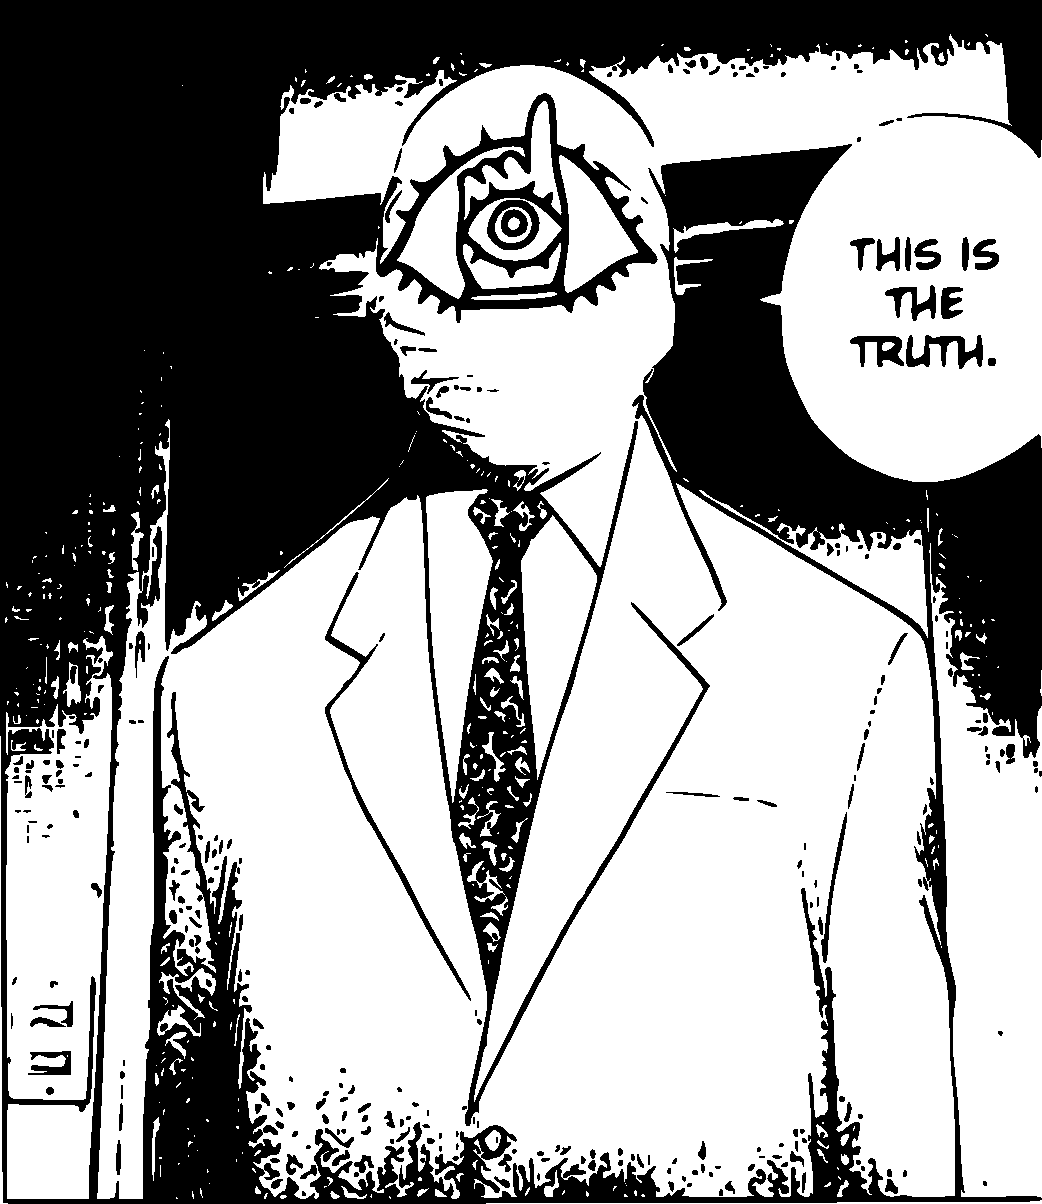
\includegraphics[width=0.4\textwidth,right ]{../../preamble/tomodachi.pdf} 
\end{figure}
\newpage %\setmainfont{Times New Roman}
\normalsize

\tableofcontents 
\newpage

%==================FOOTER e HEADER=======================%
\fancyhf{}
\fancyhead[L]{\nouppercase{\leftmark}}
\fancyhead[R]{Sezione \thesection}
\fancyfoot[C]{\thepage}
\fancyfoot[L]{\titolo}
\fancyfoot[R]{ Marco Casu}
%\fancyfoot[R]{\setmainfont{Palace Script MT}\huge Marco Casu \setmainfont{Times New Roman}}
%==================FOOTER e HEADER=======================%

%==================INIZIO======================%
\chapter{Introduzione}
\section{Basic Definitions}
In the context of the artificial intelligence, an \textbf{agent} is an entity that can\begin{itemize}
    \item Perceive the environment through \textit{sensors} (percepts)
    \item Act upon the environment through \textit{actuators} (actions).
\end{itemize}
We say that an agent is \textbf{rational} if he selects the action that maximize a given \textit{performance measure}, informally, he attempts to do ''the right thing''. The best case is hypothetical and often unattainable, because the agent usually can't perform all the actions needed, and can't perceive all the information about the environment.\bigskip

An agent has a performance measure $M$ and a set $A$ of all possible actions, given percept a sequence $A$ and knowledge $K$ (data), he has to select the next action $a\in A$, is a map\begin{equation}
    M\times P\times K \longrightarrow A.
\end{equation} 
An action $a$ is optimal if it maximize the expected value of $M$, given the sequence $P$ and the knowledge $K$. An agent is rational if he always chooses the optimal action. More specifically, an agent consists in two components:\begin{itemize}
    \item an architecture which provides an interface to the environment
    \item a program executed on that architecture.
\end{itemize}
There are some limitation that we aren't considering, such as the fact that determining the optimal choice could take too much time or memory on the architecture.

\subsection{Types of Agents}
There are different kinds of agents, a \textbf{Table Driven Agent} is the simplest form of agent architecture. It's essentially a look-up table that maps every possible sequence of percepts (what the agent has sensed so far) to a corresponding action the agent should take. His behavior can be resumed in the algorithm \ref{alg:table_agent}.

\begin{algorithm}
    \caption{Table Driven Agent}\label{alg:table_agent}
    \begin{algorithmic}
    \Require \textit{percepts}
    \State \textbf{persistent}: \textit{percepts}, a sequence, initially empty
    \State\hphantom{persistent: .} \textit{table}, a table of actions, indexed by percept sequences, initially fully specified
    \State append \textit{percept} to the end of \textit{percepts} 
    \State \textit{action}$\leftarrow$\texttt{LookUp}(\textit{percepts,table})
    \State\Return \textit{action}
    \end{algorithmic}
\end{algorithm}
\bigskip


A \textbf{Reflex Agent} consists in three components:\begin{itemize}
    \item sensors to get information from the environment
    \item a decision making process, in form of a \textit{condition-action rules}, typically looks like \texttt{IF (condition) THEN (action)}.
    \item actuators, the outputs that allow the agent to affect or change the environment.
\end{itemize}

\begin{figure}[h!]
    \centering
    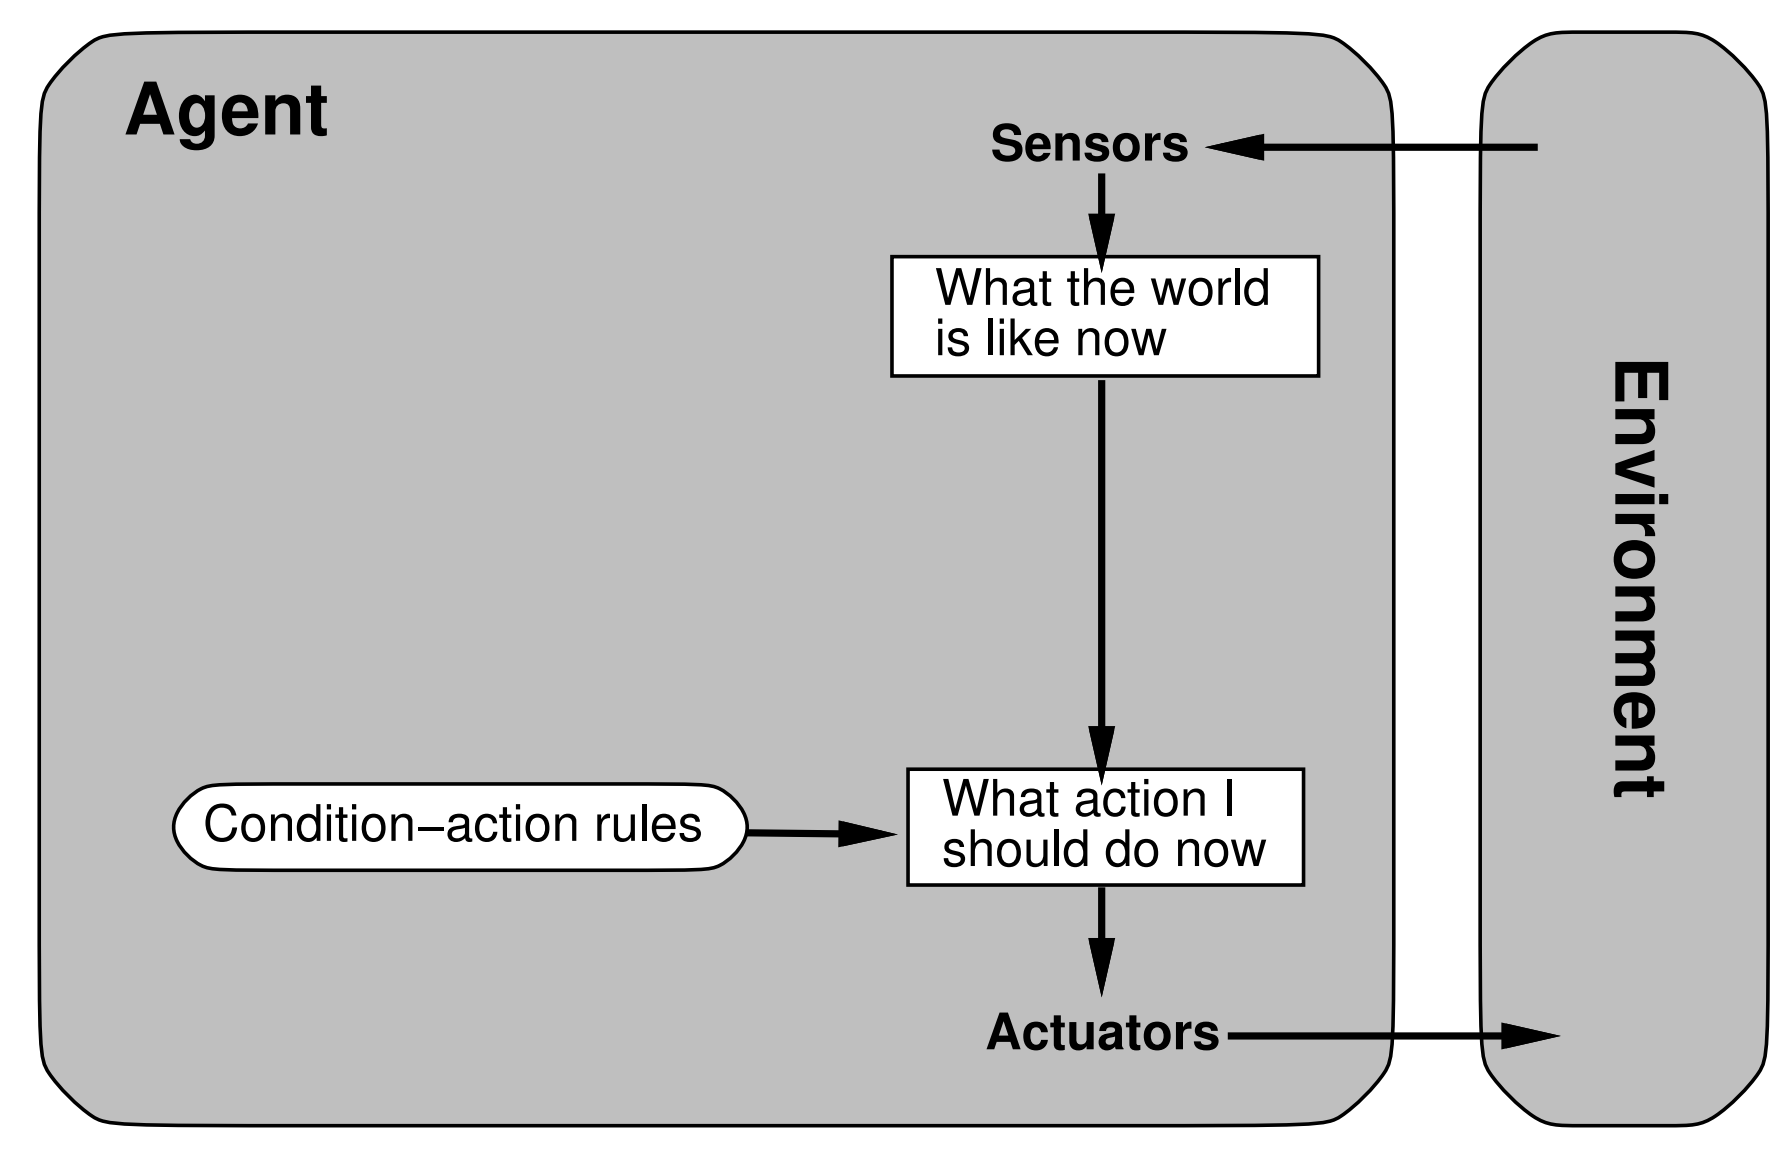
\includegraphics[width=0.4\textwidth ]{images/reflexAgent.png}
    \caption{Reflex agent diagram}
\end{figure}\bigskip

A \textbf{Model-Based Reflex Agent} is an enhanced version of the previous one, the key enhancement here is the inclusion of an \textit{Internal State} and a \textit{Model of the World} to make up for the agent's limited view of the environment. The internal state cannot simply be the last thing the agent saw; it needs to be updated to reflect reality. This is done using a Model of the World, which contains two key pieces of knowledge:\begin{itemize}
    \item 
    How the world evolves independently of the agent, his accounts for changes in the environment that occur regardless of the agent's actions (e.g., a clock ticking, an external event).
    \item
    How the agent's own actions affect the world, this is the effect of the agent's previous action (e.g., if the agent drove forward, its position changed).
\end{itemize}

\begin{figure}[h!]
    \centering
    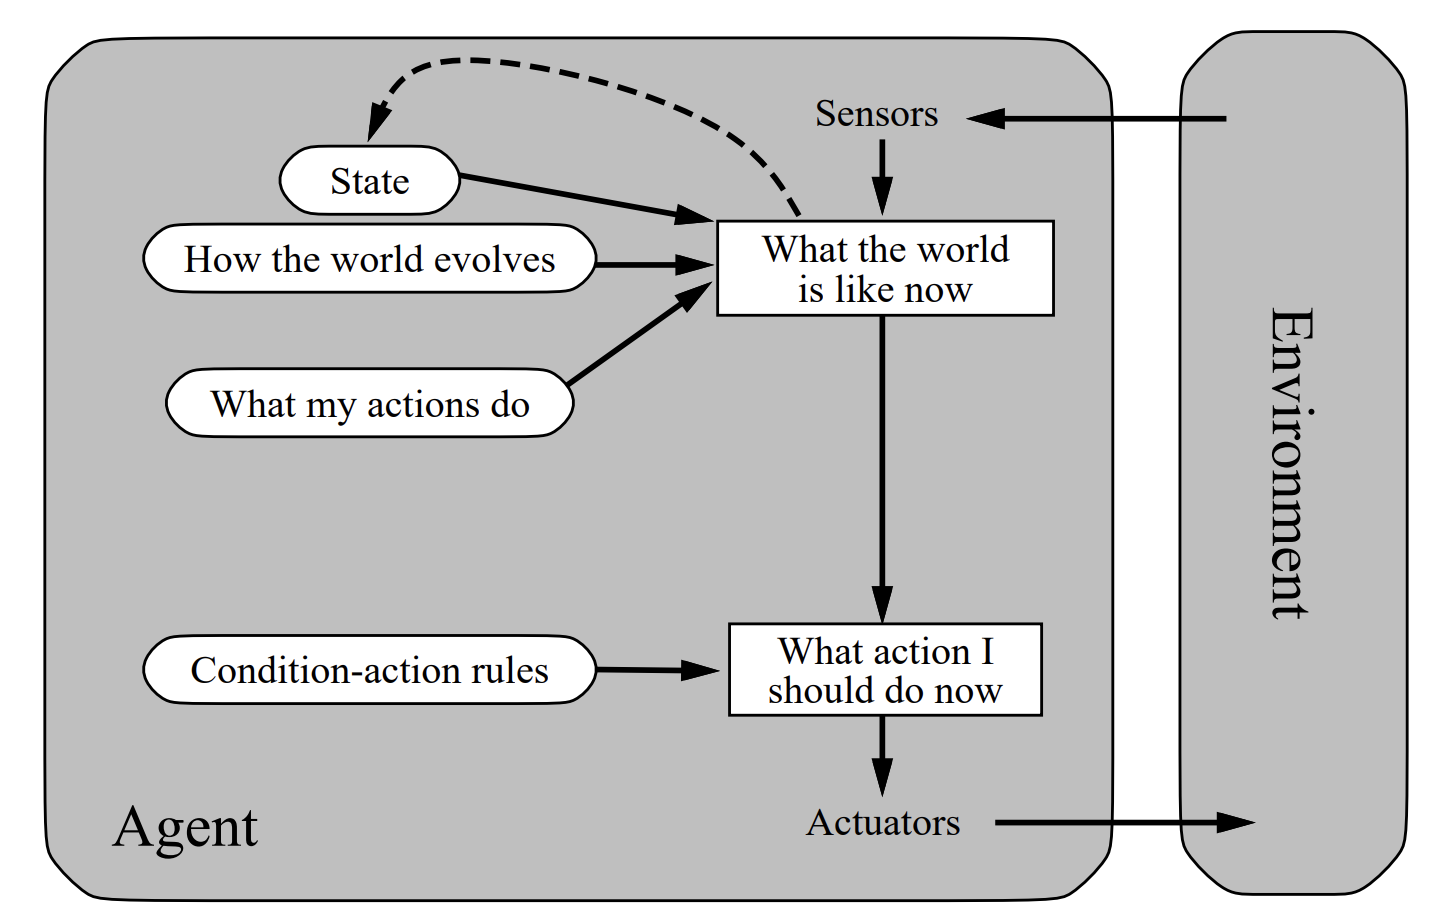
\includegraphics[width=0.4\textwidth ]{images/ModelreflexAgent.png}
    \caption{Model Based Reflex agent diagram}
\end{figure}\bigskip

If a model based reflex agent consider the future prospective, is a \textbf{Goal Based Agent}, as shown in figure \ref{img:goal_agent}.

\begin{figure}[h!]
    \centering
    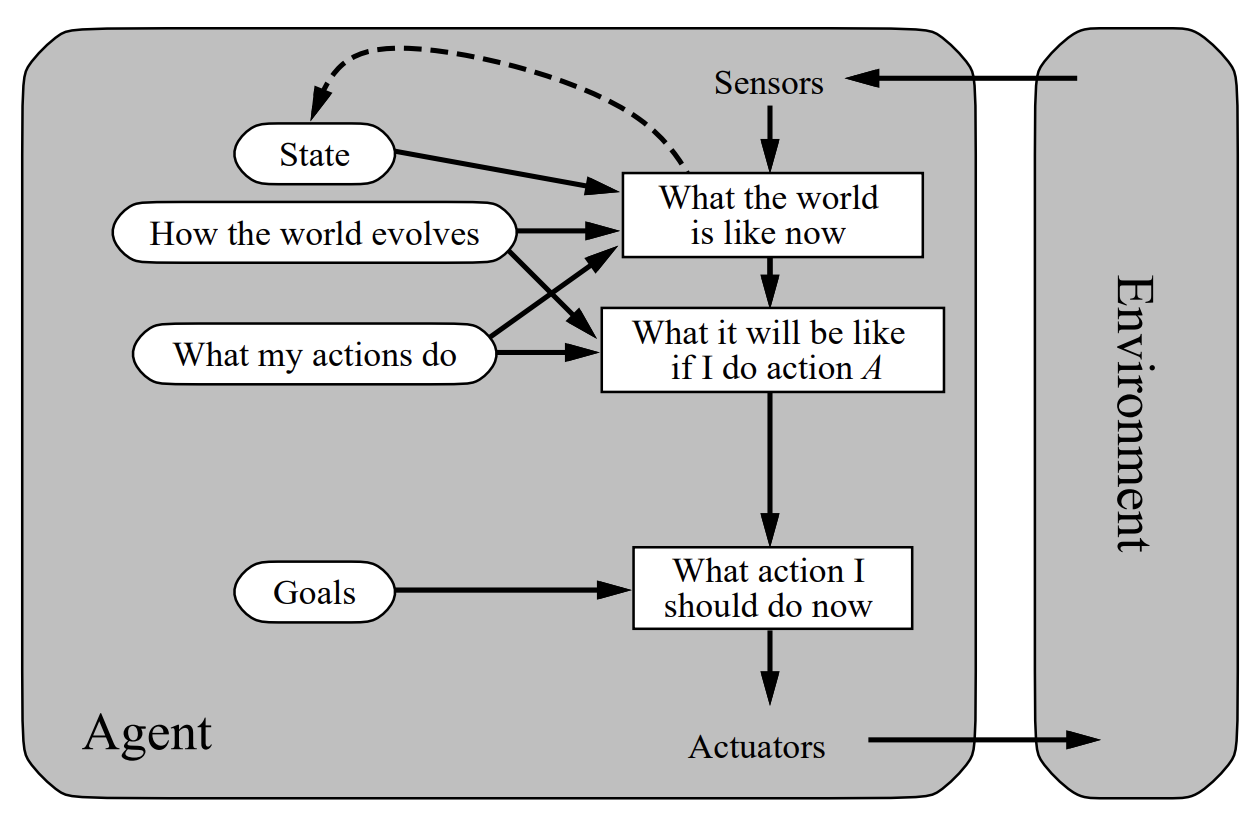
\includegraphics[width=0.4\textwidth ]{images/goal.png}
    \caption{Goal Based agent diagram}
    \label{img:goal_agent}
    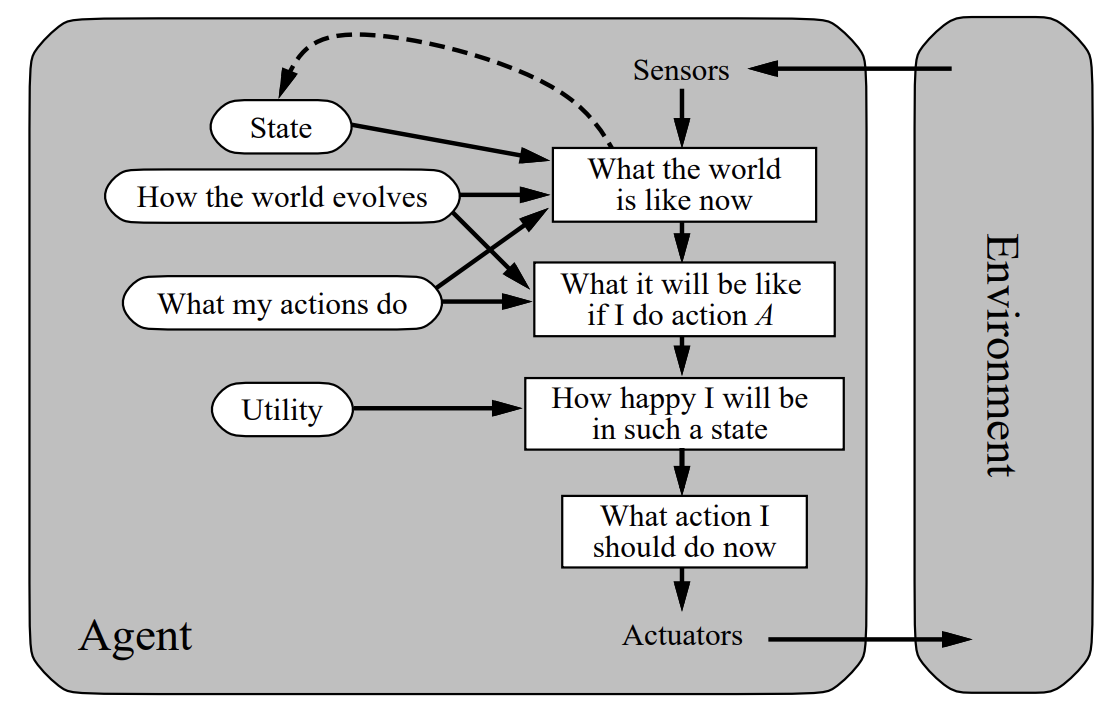
\includegraphics[width=0.4\textwidth ]{images/utility.png}
    \caption{Utility Based agent diagram}
\end{figure}\bigskip

A \textbf{Utility Based Agent} is equipped with a \textit{utility function} that maps a state to a number which represents how
desirable the state is. Agent’s utility function is an internalization of the performance function.\bigskip

A \textbf{Learning Agent} is an architecture designed to improve its efficiency over time by separating four functions:\begin{itemize}
    \item  the performance element selects actions\item  
     the critic provides feedback on those actions against a standard\item   the learning element uses this feedback to update the agent's internal knowledge\item   the problem generator suggests exploratory actions to gain new knowledge. This structure enables the agent to continuously adapt and improve its decision-making.
\end{itemize}

\begin{figure}[h!]
    \centering
    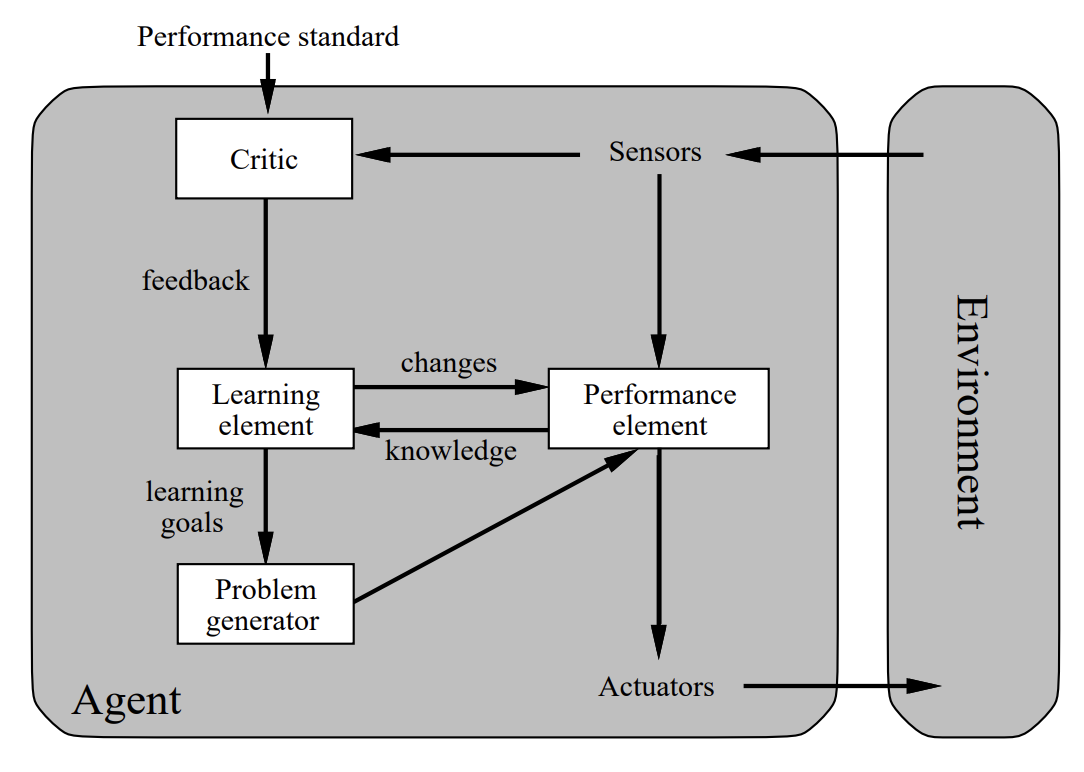
\includegraphics[width=0.4\textwidth ]{images/learn_agent.png}
    \caption{Learning agent diagram}
\end{figure}\bigskip

An agent can be classified in one of the following groups:\begin{itemize}
    \item a \textbf{domain specific agent }  is a solver specific to a particular problem (such as playing chess), is usually more efficient.
    \item a \textbf{general agent} is a solver for general problems, such as learning the rule of any board game, is usually more intelligent but less efficient.
\end{itemize}
\subsection{The Environment}
An environment can be classified in terms of different attributes:\begin{itemize}
    \item An environment can be \textbf{fully observable} if all the relevant information are accessible to the sensors, otherwise is \textbf{partially observable}.
    \item If there are no uncertainty, the environment is \textbf{deterministic}. An environment is \textbf{stochastic} if uncertainty is quantified by using probabilities, otherwise is \textbf{non deterministic} if uncertainty is managed as actions with multiple outcomes.
    \item An environment is \textbf{episodic} if the correctness of an action can be evaluated instantly, otherwise if are evaluated in the future developments, is \textbf{sequential}. 
    \item An environment can be \textbf{static} or \textbf{dynamic}, if itdoes not change, but the agent's performance
score changes, the environment is called \textbf{semi-dynamic}.
    \item An environment can be perceived as \textbf{discrete} or \textbf{continuous}.
    \item In a single environment there may be multiple agent, that can be \textbf{competitive} or \textbf{cooperative}.
\end{itemize}
Many sub-areas of AI can be classified by:\begin{itemize}
    \item Domain-specific vs. general.
    \item The environment.
    \item Particular agent architectures sometimes also play a role, especially
    in Robotics.
\end{itemize}
It follows a classification of some areas in terms of the attributes we discussed:\begin{itemize}
    \item \textbf{Classical Search}, the environment is\begin{itemize}
        \item fully observable
        \item deterministic
        \item static 
        \item sequential
        \item discrete
        \item single-agent
    \end{itemize}
    and the approach is \textit{domain specific}.
    \item \textbf{Planning}, the environment is\begin{itemize}
        \item fully observable
        \item deterministic
        \item static
        \item sequential 
        \item discrete
        \item single-agent
    \end{itemize}
    and the approach is \textit{general}.
    \item \textbf{Adversarial Search}, the environment is\begin{itemize}
        \item fully observable
        \item deterministic
        \item static 
        \item sequential    
        \item discrete
        \item multi-agent
    \end{itemize}
    and the approach is \textit{domain specific}.
    \item \textbf{General Game Playing}, the environment is\begin{itemize}
        \item fully observable
        \item deterministic
        \item static 
        \item sequential    
        \item discrete
        \item multi-agent
    \end{itemize}
    and the approach is \textit{general}.
    \item \textbf{Constraint Satisfaction \& Reasoning}, the environment is\begin{itemize}
        \item fully observable
        \item deterministic
        \item static 
        \item episodic    
        \item discrete
        \item single-agent
    \end{itemize}
    and the approach is \textit{general}.
    \item \textbf{Probabilistic Reasoning}, the environment is\begin{itemize}
        \item partially observable
        \item stochastic
        \item static 
        \item episodic    
        \item discrete
        \item single-agent
    \end{itemize}
    and the approach is \textit{general}.
\end{itemize}
\chapter{Search Problems}
\section{Classical Search}
\end{document}